\documentclass[12pt,a4paper]{article}
\usepackage{Preamble}
\usepackage{subfiles}

\begin{document}
\maketitle
{\hypersetup{linkcolor=black}\tableofcontents}

\section{Introduction}
Good circuit design is more than simply calculating the “correct” component values, it is ensuring that the circuit behaves properly when it has been manufactured in large quantities! Part of that evaluation is ensuring that the circuit performs adequately within the bounds of production tolerances. Student projects, by their nature, are often one-off designs, and students have the ability to adjust component values to account for outputs that are not quite what was expected. In a production setting, this is not a feasible strategy.

This project will produce a front-end for the Spice circuit simulator that supports the testing of designs across the range of possible production values of components. The input to the simulator will be a Spice simulation file (previously tested using a package such as LTSpice), and a set of component tolerances. The project will then proceed to run the simulation multiple times, for the different component tolerances, to test out the impact of these on the final output.

\section{Installation}
\begin{itemize}
    \item \textbf{Requirement}\par
    ngspice = 34\par
    python3\par
    Module: numpy, scipy, PyQt5 $\geqslant$ 5.15, matplotlib, pandas, django, quantiphy\par
    Optional Module: bs4, weasyprint, coloredlogs\par

    \item  \textbf{Ngspice Configuration}\par
    Ngspice should be installed in directory \textit{./Workspace}. This project has included a pre-compiled ngspice. If anything wrong is with it, you can compile it by yourself. It can be downloaded from \href{https://sourceforge.net/projects/ngspice/}{sourceforge ngspice Git page}.

    To compile ngspice34, make sure you enable the relative paths for spinit and code models.
    \lstset{backgroundcolor=\color{white},numbers=none,keepspaces=false}
    \begin{lstlisting}
    $ ./configure --enable-relpath
    \end{lstlisting}

    The normal compile command for linux-64 bit installed is
    \begin{lstlisting}{language=bash}
    $ sudo apt install libxaw7-dev autoconf automake libtool libreadline6-dev
    $ ./autogen.sh
    $ mkdir release
    $ cd release
    $ ../configure --with-x --enable-xspice --enable-cider --with-readline=yes --enable-openmp --enable-relpath --prefix={Path-To-Workspace} --disable-debug CFLAGS="-m64 -O2" LDFLAGS="-m64 -s"
    $ make clean
    $ make install
    \end{lstlisting}
    Where Path-To-Workspace is the complete path to the dirctory \textit{Workspace}.
\end{itemize}

\section{Flowchart}
\begin{figure}[ht]
    \centering
    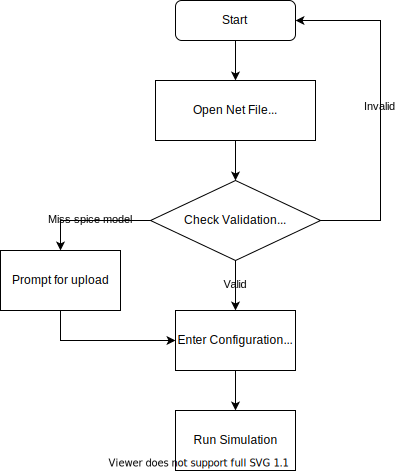
\includegraphics{Image/spice.pdf}
    \caption{}
\end{figure}

\section{Project structure}
This project is mainly written in python3 and for circuit analysis part, it is written in spice language.

\subsection{main.py}
Main function of the project.

\noindent\textbf{Variable Description}
\begin{itemize}
    \item \textcolor{blue}{root}: Root path of main.python3
    \item \textcolor{blue}{path}: PATH variable of the system
    \item \textcolor{blue}{spiceinit}: See Function \hyperlink{init}{init()} in Logging.py for more information.
\end{itemize}

\subsection{src/read.py}
Read in a circuit file

\begin{itemize}[leftmargin=*]
    \item \textcolor{blue}{rm(*filename)}\\
        Delete the given files. If the file does not exist, pass.

    \item Class \textcolor{blue}{C}\\
        Capacitor.\\
        \textbf{Attribute:}
        \begin{itemize}
            \item \textcolor{blue}{C.name}: Capacitor name
            \item \textcolor{blue}{C.c}: Capacitance value
            \item \textcolor{blue}{C.tol}: Capacitor tolerance
        \end{itemize}

    \item Class \textcolor{blue}{R}\\
        Capacitor.\\
        \textbf{Attribute:}
        \begin{itemize}
            \item \textcolor{blue}{R.name}: Resistor name
            \item \textcolor{blue}{R.r}: Resistance value
            \item \textcolor{blue}{R.tol}: Resistor tolerance
        \end{itemize}

    \item Class \textcolor{blue}{circuit}\\
        Circuit class.\\
        \textbf{Attribute:}
        \begin{itemize}
            \item Initialize\\
                Give the file name of the netlist file. For example, circuit(TIA.cir)

            \item \textcolor{blue}{circuit.read()}\\
                Read in the netlist and create two circuit files, \textit{test.cir} and \textit{run.cir}.

                Acceptable control command in netlist: ".model", ".subckt", ".global", ".include", ".lib", ".temp", ".ends", ".ac", ".probe"

                \textbf{Caution:} All commands between \textbf{.control} and \textbf{.endc} will be ignored.

                To run simulation correctly, the netlist must have a net named \textbf{"out"}!

            \item \textcolor{blue}{circuit.init()}\\
                Initialize the circuit, check if any error in circuit file.

                It will call the ngspice to first perform an operating point analysis. During this process, it will give us all the component and net information. The first perform output data is stored in file \textit{'op'} abd \textit{'list'}.

                If the operation point analysis is passed, it will perform an AC, small-signal frequency response
                analysis and the output data is stored in file \textit{'ac'}.

                Finally, it will read the information of the resistors and capacitors in the circuit from file 'list', generated during the first test. The components in the subcircuit will not be read.

                \textbf{Return:} two-element tuple (error\textunderscore message, flag).

                flag=0: no error occurs or uncategorized error

                flag=1: include file error. Could not find include file

                flag=2: Unknown subcircuit error.

                If no error occur, both elements are 0.

            \item \textcolor{blue}{circuit.fixinclude(self, repl, mode)}\\
                Fix the error, missing the include file or subcircuit file.

                \textbf{Parameters:}\\
                repl: String, Required. Uploaded include file\\
                mode: Int, Required. 1 or 2. 1 represents include file error, 2 represents subcircuit error.

            \item \textcolor{blue}{circuit.readnet()}\\
                Read the nets of circuit of file 'op'. Nets in the subcircuit will not be read.
\end{itemize}

\subsection{src/\textunderscore write.py}
Write control files. This is the sub-file for class \textcolor{blue}{circuit}, defining new attributes.

\begin{itemize}[leftmargin=*]
    \item \textcolor{blue}{circuit.create\textunderscore prerun()}\\
        Create the control file \textit{run\textunderscore control \textunderscore pre.sp}. It tests the circuit before the formal simulation. Measuring max and min gain does not require this function to run.

    \item \textcolor{blue}{circuit.create\textunderscore sp(add=False)}\\
        Create the main simulation control file \textit{run\textunderscore control.sp}

    \item \textcolor{blue}{circuit.create\textunderscore wst()}\\
        Create the control file \textit{run\textunderscore control\textunderscore wst.sp} for the worst case simulation.

    \item \textcolor{blue}{circuit.create\textunderscore step()}\\
        Create the control file \textit{run\textunderscore control.sp} for the step mode.

    \item \textcolor{blue}{circuit.create\textunderscore opamp()}\\
        Create the control file \textit{run\textunderscore control.sp} for switching op amp.

    \item \textcolor{blue}{circuit.create\textunderscore cmrr(add=False)}\\
        Create the control file \textit{run\textunderscore control.sp} and \textit{run\textunderscore control\textunderscore wst.sp} for CMRR mode.

        If add=True, control file \textit{run\textunderscore control\textunderscore wst.sp} will not be created as it would have been run when first created.

\end{itemize}

\subsection{src/\textunderscore resultaly.py}
Analyse simulation results and create report. This is the sub-file for class \textcolor{blue}{circuit}, defining new attributes.

\begin{itemize}
    \item \textcolor{blue}{circuit.resultdata(self, worst=False, add=False, mode=None)}\\
        Analyse simulation results.

        Parameters:

        worst: Bool, Optional\par
        \quad If true, it will analyse the worst case simulation data.

        add: Bool, Optional\par
        \quad If true, this function read in data from last end read point.

        mode: Str, Optional\par
        \quad This function would analyse data using importance sampling by default.

        \quad Available choice: 'Opamp' and 'Step'

    \item \textcolor{blue}{f(x, miu, sigma, tol)}\\
        Importance sampling function. It converts uniform distribution sampling data back to Gaussian distribution data, where \textit{miu}($\mu$) is the mean of the distribution, \textit{sigma}($\sigma$) is the standard deviation and \textit{tol} is the tolerance. This function calculates:
        \begin{equation*}
            \frac{\exp\left [\frac{(x-\mu)^2}{2\sigma^2}\right ]}{\frac{\text{erf}(\frac{tol\cdot\mu}{\sqrt{2}\sigma\pi})-\text{erf}(\frac{tol\cdot\mu}{\sqrt{2}\sigma\pi})}{2}\sqrt{2\pi}\sigma}
        \end{equation*}

    \item \textcolor{blue}{circuit.report(mode=None)}\\
        Generate html5 report. This function is run in another thread.
\end{itemize}

\subsection{src/plot.py}
Code for GUI interface.

\textbf{Class \textcolor{blue}{plotGUI(QtWidgets.QMainWindow)}}

Main GUI interface.

\begin{itemize}
    \item UI file: main.ui\par
        To edit this file, you can install module qt5-applications by
        \lstset{backgroundcolor=\color{white},numbers=none,keepspaces=false}
        \begin{lstlisting}
        pip install qt5-applications
        \end{lstlisting}

        Open the designer in Path-To-site-packages/qt5\textunderscore applications/Qt/bin/designer and edit it.

        The varibles for the main widgets of this window is shown in the Figure \ref{Main} below.
        \begin{figure}[ht]
            \centering
            \includegraphics[width=0.9\textwidth]{Image/main.eps}
            \caption{Definition of the main window}
            \label{Main}
        \end{figure}


    \item \textcolor{blue}{openfile()}\\
        Open a new netlist file. If there is a new opened, warn the user with a message box.\label{}

        It will first copy the selected file to a new folder, named with the filename and uploaded time. Then, call the function to read the file. If no error occur, call the function to initialize the circuit. If some error happens, it will pop out a window. Finally, show the configuration window.

    \item \textcolor{blue}{configCreate()}\\
        Read in parameters from configuration window. Check the validity of the parameters and call specific function to create control files.

    \item \textcolor{blue}{configreject()}\\
        If 'cancel' is clicked in the configuration window, this function will run if the signal is connected to this function.

    \item \textcolor{blue}{start\textunderscore process(finishmode, runmode=0)}\\
        Call ngspice to do simulation.

        Parameters:

        \quad finishmode: String, Required

        \quad Available options:

        \quad runmode: int, optional

        \quad runmode=0, run only run\textunderscore control.sp

        \quad runmode=1, run both run\textunderscore control.sp and run\textunderscore control\textunderscore wst.sp

    \item \textcolor{blue}{kill()}\\
        Kill the ngspice if \textit{Cancel} is clicked while it is running.

    \item \textcolor{blue}{finishrun(mode)}\\
        This function will be run when ngspice simulation is finished. It checks if any error occurs during ngspice processing. Then, it will call function \textcolor{blue}{postinit()}.

        mode: String, Required. It determines which method the result data would be processed.

    \item \textcolor{blue}{postinit(mode=None)}\\
        Do some post-initialization after running simulation. It will enable and disable certain buttons or widgets on the main based on the given mode.

    \item \textcolor{blue}{plot(mode=None)}\\
        Plot the data on the main window based on the given mode.

    \item \textcolor{blue}{plotwst()}\\
        Plot the worst case data.

    \item \textcolor{blue}{AddTime()}\\
        Add more simulation time. This function will run when 'enter' is pressed.

    \item \textcolor{blue}{calcp()}\\
        Calculate the y axis value. This function will run when 'enter' is pressed.

    \item \textcolor{blue}{analy()}\\
        If the button analysis is clicked, show the configuration window.

    \item \textcolor{blue}{reset()}\\
        If the reset button is clicked, clear the figure.

\end{itemize}

\subsection{src/\textunderscore subwindow.py}
Define the Processing window and configuration window.

\begin{itemize}
    \item Class \textcolor{blue}{processing(QtWidgets.QDialog)}\\
        Show the processing dialog while ngspice simulation is running.

        ui file: src/processing.ui

    \item Class \textcolor{blue}{config(QtWidgets.QDialog)}\\
        Configuration window definition.

        ui file: src/config.ui

        Variable definition of this window is shown in the figure \ref{Config} below.
        \begin{figure}[ht]
            \centering
            \begin{subfigure}[b]{0.9\textwidth}
                \centering
                \includegraphics[width=1\textwidth]{config.eps}
                \caption{Simulation tab}\vspace{1ex}
            \end{subfigure}
            \begin{subfigure}[b]{0.9\textwidth}
                \centering
                \includegraphics[width=1\textwidth]{config34.eps}
                \caption{CMRR and Op amp tab}\vspace{1ex}
            \end{subfigure}
            \caption{Configuration window definition}
            \label{Config}
        \end{figure}

\end{itemize}


\subsection{src/MplWidget.py}
The header file for the plotting area of both configuration window and main window.

\subsection{src/Logging.py}
Log file definition and some initialization of the tool.

\begin{itemize}
    \item \textcolor{blue}{check\textunderscore module(module\textunderscore name)}\\
        Check if the given module is installed. If the given module exists, return the module name. Otherwise, return none.

        Parameters:

        module\textunderscore name: String, Required

    \item \textcolor{blue}{import\textunderscore module(module\textunderscore name, attr=None)}\\
        Import the module. If attr is given, import the attribute from the module.

        Parameters:

        module\textunderscore name: String, Required

        attr: String or list, Optional

    \item \textcolor{blue}{\hypertarget{init}{init(check=True)}}\\
        Do md5sum check of the software ngspice and check if the  user defined configuration file for ngspice '.spiceinit' is correct.

        '.spiceinit' is located at the HOME dirctory typically. To edit the default content of this file, you can edit it in file Workspace/.spiceinit . Each time when the tool starts, it will check if these two file are the same.

        Parameters:

        check: Bool, Optional. Default value: True. Whether to perform md5sum check of ngspice.

        Return: string. The content in the file '.spiceinit' in the HOME dirctory. If the file does not exist, return False.
\end{itemize}

\end{itemize}


\section{GUI Guide}
\subsection{Main Window}
The interface of the main window is shown in figure \ref{Main}.

The addtimetext line is enabled if the analysis is not step mode or Op amp mode.

The probability probe is also disabled under Op amp mode.

\subsection{Configuration Window}
The interface of the configuration window is shown in figure \ref{Config}.

For tolerance analysis, you can enter the simulation options in the first tab and enter the tolerance of each component in the second tab \textit{Tolerance}. Then click OK under either first or second tab.

For CMRR analysis, enter the simulation options under the third tab \textit{CMRR} and confirm the tolerance under the second tab. Then click OK under the third tab. If you click under the tolerance tab, it will perform the simulation options of the first tab.

For Op amp alteration, enter the simulation options and click OK both under the fourth tab.

\subsection{Report}
To see html5 report, under the directory src/report, run the below command.
\lstset{backgroundcolor=\color{white},numbers=none,keepspaces=false}
\begin{lstlisting}
    python3 -m manage.py runserver
\end{lstlisting}

Then open 127.0.0.1:8000, you can see the result report.

Or you can find the html5 code file under src/htmlreport/templates/report.html

If you have the module weasyprint installed, you can find the pdf report under the circuit file base directory in folder Workspace.


\bibliographystyle{agsm}
%\bibliography{}

\end{document}